\chapter{非线性偏微分方程：演化、守恒律与可积结构}
\label{chap:nonlinear-pde}

线性理论的核心优势是叠加原理与谱分解；非线性问题失去这一结构以后，首先需要回答的不是“能否猜到一个孤子”，而是三个更基本的问题：初值是否在有限时间内决定唯一解，光滑解失效后应怎样定义弱解，以及耗散、色散与 Hamilton 结构分别如何控制长期演化。本章先从抽象演化方程和守恒律建立母结构，再讨论 Burgers 与 KdV 所代表的耗散/色散正则化，最后进入 Lax 对、反散射和 NLS。具体可积模型始终位于一般演化与近似尺度之后。

\section{一般非线性演化、特征线与弱解}
\label{sec:nonlinear-evolution-general}

接下来考察从精确演化方程到 mild solution。

设 \(X\) 是 Banach 空间，非线性演化问题写成
\begin{equation}
\frac{\dd u}{\dd t}=Au+F(u),
\qquad
u(0)=u_0,
\label{eq:abstract-semilinear-evolution}
\end{equation}
其中 \(A:D(A)\subset X\to X\) 是可能无界的线性算子，\(F\) 是非线性映射。若 \(A\) 生成强连续半群 \(S(t)=\ee^{tA}\)，则与直接对 \(A\) 求逆相比，更稳健的形式精确表达是 Duhamel 公式
\begin{equation}
\boxed{
 u(t)=S(t)u_0+
 \int_0^tS(t-s)F(u(s))\,\dd s
 }.
\label{eq:duhamel-semilinear}
\end{equation}
满足\eqnrefs{eq:duhamel-semilinear} 的连续函数称为 mild solution。若它还落在 \(D(A)\) 中并具有足够时间正则性，才可进一步称为 classical solution。这个区分在热方程、Navier--Stokes、NLS 等无界生成元问题中很重要：形式上的 \(u_t=Au+F(u)\) 并不自动保证 \(Au\) 逐点有意义。

局部适定性的标准输入是：在某个半径 \(R\) 的球上，\(F\) 局部 Lipschitz，且半群满足
\[
\|S(t)\|\le M\ee^{\omega t}.
\]
此时对足够短的时间区间，\eqnrefs{eq:duhamel-semilinear} 的右端定义一个压缩映射，于是存在唯一 mild solution。真正的难点因此被分成两部分：线性生成元决定传播估计，非线性项决定 Lipschitz 或更精细的 multilinear 估计。

\begin{derivation}[Duhamel 公式与局部压缩映射]
先假设 \(u\) 是 classical solution，并固定终点 \(t>0\)。对参数 \(s\in[0,t]\) 定义
\[
w(s):=S(t-s)u(s).
\]
这个写法只使用正时间半群，不要求 \(S(t)\) 可逆。若 \(u(s)\in D(A)\)，由生成元定义和半群在 \(D(A)\) 上与 \(A\) 的相容性，
\[
\begin{aligned}
\frac{\dd}{\dd s}w(s)
&=-AS(t-s)u(s)+S(t-s)\dot u(s)\\
&=-S(t-s)Au(s)+S(t-s)\bigl(Au(s)+F(u(s))\bigr)\\
&=S(t-s)F(u(s)).
\end{aligned}
\]
从 \(s=0\) 积分到 \(s=t\)，得到
\[
u(t)-S(t)u_0
=\int_0^tS(t-s)F(u(s))\,\dd s,
\]
这正是\eqnrefs{eq:duhamel-semilinear}。因此 Duhamel 公式对一般强连续半群成立，并不需要人为引入不存在的 \(S(-t)\)。

现在在 \(C([0,T],X)\) 上定义
\[
(\Phi u)(t)
=S(t)u_0+
\int_0^tS(t-s)F(u(s))\,\dd s.
\]
若 \(u,v\) 都落在半径 \(R\) 的球内，而 \(F\) 在该球上的 Lipschitz 常数为 \(L_R\)，则
\[
\begin{aligned}
\|\Phi u-\Phi v\|_{C_T}
&\le
\sup_{0\le t\le T}
\int_0^t
M\ee^{\omega(t-s)}
L_R\|u(s)-v(s)\|\,\dd s\\
&\le
ML_R T\ee^{\omega_+T}
\|u-v\|_{C_T},
\end{aligned}
\]
其中 \(\omega_+=\max(\omega,0)\)。只要
\[
ML_RT\ee^{\omega_+T}<1,
\]
\(\Phi\) 就是压缩映射。再把 \(T\) 取得足够小，使 \(\Phi\) 把选定闭球映回自身，Banach 不动点定理给出唯一局部 mild solution。这个证明同时说明局部存在时间由初值范数、半群增长和非线性 Lipschitz 常数共同控制。
\end{derivation}


接下来考察最大解、延拓准则与能量闭合。

局部不动点只说明短时间存在，不能自动推出解能延伸到任意时刻。设\eqnrefs{eq:abstract-semilinear-evolution}在初值 $u_0$ 下的唯一 mild solution 定义在最大时间区间
\[
0\le t<T_{\max}.
\]
在 $F$ 对有界集局部 Lipschitz 的标准情形，有限时间失效必须伴随解离开所有可继续使用局部存在定理的有界集。最常用的延拓判据写成
\begin{equation}
T_{\max}<\infty
\quad\Longrightarrow\quad
\limsup_{t\uparrow T_{\max}}\|u(t)\|_X=\infty,
\label{eq:semilinear-blowup-alternative}
\end{equation}
只要 $F$ 在整个 $X$ 上定义且其局部 Lipschitz 常数只依赖球半径。若方程只在某个开子集 $\mathcal U\subset X$ 上定义，则结论应改为：当 $t\uparrow T_{\max}$ 时，$u(t)$ 必须离开 $\mathcal U$ 中的每个相对紧子集。这个版本比简单写“范数爆炸”更一般。

\begin{derivation}[局部适定性怎样给出 blow-up alternative]
用反证法证明：若 \(T_{\max}<\infty\) 且解有界，则可延拓过 \(T_{\max}\)，矛盾。

\emph{第一步：假设有界。}设 \(T_{\max}<\infty\)，但存在常数 \(R<\infty\) 使
\[
  \sup_{0\le t<T_{\max}}\|u(t)\|_X\le R.
\]

\emph{第二步：统一存在时间。}取任意序列 \(t_n\uparrow T_{\max}\)。所有 \(u(t_n)\) 位于半径 \(R\) 的球内。\(F\) 在半径 \(R+1\) 的球上具有统一 Lipschitz 常数 \(L_{R+1}\) 和界 \(M_{R+1}\)。局部压缩映射证明给出的存在时间仅依赖这些参数：
\[
  \tau=\tau(R,M_{R+1},\omega,L_{R+1})>0,
\]
与具体初值 \(u(t_n)\) 和起始时刻 \(t_n\) 无关。

\emph{第三步：重启并延拓。}把 \(u(t_n)\) 当作新的初值，从 \(t_n\) 重新启动积分方程
\[
  u(t)=S(t-t_n)u(t_n)+\int_{t_n}^t S(t-s)F(u(s))\,\dd s.
\]
局部适定性给出定义在 \([t_n,t_n+\tau]\) 上的唯一 mild solution \(v_n(t)\)。

\emph{第四步：唯一性拼接。}在重叠区间 \([t_n,T_{\max})\) 上，\(u(t)\) 和 \(v_n(t)\) 满足同一积分方程且同一初值 \(u(t_n)\)。由局部唯一性，\(u(t)=v_n(t)\) 对所有 \(t\in[t_n,T_{\max})\) 成立。

\emph{第五步：矛盾。}取 \(n\) 足够大使 \(t_n+\tau>T_{\max}\)（因 \(t_n\to T_{\max}\) 且 \(\tau>0\) 固定）。则 \(v_n\) 把 \(u\) 延拓到 \(T_{\max}\) 之后：
\[
  \tilde u(t)=\begin{cases}u(t),&0\le t<T_{\max},\\ v_n(t),&t_n\le t\le t_n+\tau.\end{cases}
\]
由第四步，拼接在 \([t_n,T_{\max})\) 上一致，故 \(\tilde u\) 是 \([0,t_n+\tau]\) 上的 mild solution，其存在时间超过 \(T_{\max}\)，与 \(T_{\max}\) 的最大性矛盾。因此若 \(T_{\max}<\infty\)，解不可能保持有界，即\eqnrefs{eq:semilinear-blowup-alternative}。

\emph{举例：热方程的全局存在。}取 \(X=L^2(\RR^n)\)，\(A=\Delta\)，\(F(u)=-u^3\)。能量估计给出
\[
\frac12\frac{\dd}{\dd t}\|u\|_{L^2}^2
=-\|\nabla u\|_{L^2}^2-\int u^4\,\dd x
\le0,
\]
故 \(\|u(t)\|_{L^2}\le\|u_0\|_{L^2}\) 一致有界，blow-up alternative 给出全局存在。

\emph{举例：非线性爆破。}对 ODE \(u'=u^2\)，\(u(0)=u_0>0\)，解 \(u(t)=u_0/(1-tu_0)\) 在 \(T_{\max}=1/u_0\) 爆破，\(\|u(t)\|\to\infty\) 符合判据。

\emph{举例：波方程的能量守恒。}取 \(X=H^1(\RR^3)\times L^2(\RR^3)\)，方程 \(\dd_t^2 u-\Delta u=0\)。能量
\[
E(t)=\frac12\int(|\dot u|^2+|\nabla u|^2)\,\dd x
\]
守恒，$\|u(t)\|_X\le C\|u_0\|_X$ 一致有界，全局存在。

\emph{推广与物理建模。}在流体力学中，Navier--Stokes 方程的 \(H^s\) 能量估计给出
\[
\frac{\dd}{\dd t}\|u\|_{H^s}\le C\|u\|_{H^s}^{1+2/(s-1)},
\]
blow-up alternative 把 Millennium 问题“解是否全局存在”等价为“\(\|u(t)\|_{H^s}\) 是否在有限时间爆破”。在量子场论中，经典 Yang--Mills 方程的 blow-up 分析决定规范场是否在有限时间形成 singularity，这与色禁闭机制相关。在广义相对论中，Einstein 方程的 Cauchy 问题通过能量估计与 blow-up alternative 给出局部存在性，全局存在性至今仍是开放问题。
\end{derivation}

在 Hilbert 空间中，延拓问题常通过能量估计闭合。设内积对第一变量线性，并假设 classical solution 满足
\[
\operatorname{Re}\langle Au,u\rangle
\le a\|u\|^2,
\qquad
\operatorname{Re}\langle F(u),u\rangle
\le b_0+b_1\|u\|^2.
\]
则
\[
\begin{aligned}
\frac12\frac{\dd}{\dd t}\|u(t)\|^2
&=\operatorname{Re}\langle Au+F(u),u\rangle\\
&\le b_0+(a+b_1)\|u\|^2.
\end{aligned}
\]
令 $c=a+b_1$。Gronwall 不等式给出
\begin{equation}
\|u(t)\|^2
\le
\begin{cases}
\ee^{2ct}\|u_0\|^2+
\dfrac{b_0}{c}\bigl(\ee^{2ct}-1\bigr),&c\ne0,\\[8pt]
\|u_0\|^2+2b_0t,&c=0.
\end{cases}
\label{eq:semilinear-energy-gronwall}
\end{equation}
因此，一旦局部理论的延拓准则只要求控制 $\|u\|_X$，这种先验能量界就能把局部解推进为全局解。更困难的 PDE 中，真正工作往往正是寻找一个足够强、又能被方程本身控制的能量泛函。

接下来考察一阶守恒律、特征线与经典解失效。

一维标量守恒律的母式是
\begin{equation}
u_t+\partial_x f(u)=0,
\label{eq:scalar-conservation-law}
\end{equation}
其中 \(f\) 为 flux。只要 \(u\) 光滑，就可写成
\[
u_t+f'(u)u_x=0.
\]
沿特征线 \(x=x(t)\) 取
\[
\dot x=f'(u),
\]
则
\[
\frac{\dd}{\dd t}u(x(t),t)
=u_t+\dot x\,u_x=0.
\]
因此振幅沿特征线保持不变，而传播速度依赖振幅本身。正是这种“不同振幅以不同速度传播”的机制导致特征线可能在有限时间交叉，并使 \(u_x\) 发散。

一旦 classical solution 失效，守恒律仍可在分布意义下成立。称 \(u\in L^1_{\mathrm{loc}}\) 为弱解，若对任意 \(\phi\in C_c^\infty\) 都有
\[
\int\!\!\int
\bigl(u\phi_t+f(u)\phi_x\bigr)\,\dd x\dd t
+
\int u_0(x)\phi(x,0)\,\dd x
=0.
\]
弱解允许跳跃，但不唯一；物理解还需 entropy condition。对凸 flux，可用任意凸 entropy \(\eta(u)\) 与对应 entropy flux \(q'(u)=\eta'(u)f'(u)\) 要求
\begin{equation}
\partial_t\eta(u)+\partial_xq(u)\le0
\label{eq:entropy-inequality}
\end{equation}
按分布理解。这个不等式把“不可逆耗散方向”加入纯守恒方程，从而选出唯一 entropy solution。


接下来考察Sobolev 能量法、延拓判据与熵半群。

抽象 Banach 空间中的局部 Lipschitz 条件很清楚，但对真正的拟线性 PDE，非线性通常包含导数，不能把 $F$ 直接看成同一个 Sobolev 空间上的局部 Lipschitz 映射。此时局部适定性的核心输入是 Sobolev 代数性质与交换子估计。

在 $\RR^d$ 或紧致 $d$ 维流形上，若
\[
s>\frac d2,
\]
则 $H^s$ 连续嵌入 $L^\infty$，并且 $H^s$ 是乘法代数：
\begin{equation}
\boxed{
\|uv\|_{H^s}
\le C_s\|u\|_{H^s}\|v\|_{H^s}
}.
\label{eq:sobolev-algebra}
\end{equation}
更精细的 Moser 型估计允许把最高阶导数只放在一个因子上：
\[
\|uv\|_{H^s}
\le C_s\bigl(
\|u\|_{L^\infty}\|v\|_{H^s}
+\|v\|_{L^\infty}\|u\|_{H^s}
\bigr).
\]
若 $F\in C^{\lceil s\rceil+1}$ 且 $F(0)=0$，则在 $u\in H^s\cap L^\infty$ 的有界集上
\[
\|F(u)\|_{H^s}
\le C(\|u\|_{L^\infty})\|u\|_{H^s}.
\]
这就是把点态非线性提升到函数空间非线性的基本机制。

对一阶拟线性方程
\[
u_t+a(u)\cdot\nabla u=F(u),
\]
真正危险的是输运项中的一个空间导数。令 $\Lambda^s=(I-\Delta)^{s/2}$，对方程施加 $\Lambda^s$ 并与 $\Lambda^su$ 配对：
\[
\frac12\frac{\dd}{\dd t}\|u\|_{H^s}^2
=
-\langle \Lambda^s(a(u)\cdot\nabla u),\Lambda^su\rangle
+\langle\Lambda^sF(u),\Lambda^su\rangle.
\]
把最高阶部分拆成
\[
\Lambda^s(a\cdot\nabla u)
=a\cdot\nabla\Lambda^su
+[\Lambda^s,a]\cdot\nabla u.
\]
第一项分部积分后只留下 $\nabla\cdot a$，第二项由 Kato--Ponce/Moser 交换子估计控制。若
\[
s>\frac d2+1,
\]
则 $H^s\hookrightarrow W^{1,\infty}$，最终得到典型能量不等式
\begin{equation}
\boxed{
\frac{\dd}{\dd t}\|u(t)\|_{H^s}
\le
C\bigl(1+\|u(t)\|_{W^{1,\infty}}\bigr)
\|u(t)\|_{H^s}
}.
\label{eq:quasilinear-sobolev-energy}
\end{equation}
所以拟线性 PDE 的自然延拓判据通常不是 $\|u\|_{H^s}$ 自身先发散，而是更低阶的 Lipschitz 控制量先失控。只要
\[
\int_0^T\|u(t)\|_{W^{1,\infty}}\,\dd t<\infty,
\]
Gronwall 就能保持 $H^s$ 范数有限，从而继续 classical solution。Euler 方程的 Beale--Kato--Majda 判据正是这一思想的更精细版本。

\begin{derivation}[一阶输运项为何只损失一个 Lipschitz 范数]
先看整数 $s=m$。对每个 $|\alpha|\le m$，由 Leibniz 法则展开
\[
D^\alpha(a\cdot\nabla u)
=a\cdot\nabla D^\alpha u
+\sum_{0<\beta\le\alpha}
C_{\alpha\beta}(D^\beta a)\cdot\nabla D^{\alpha-\beta}u.
\]
与 $D^\alpha u$ 作 $L^2$ 配对。最高阶输运项满足
\[
\begin{aligned}
-\int D^\alpha u\,
 a\cdot\nabla D^\alpha u\,\dd^dx
&=-\frac12\int a\cdot\nabla|D^\alpha u|^2\,\dd^dx\\
&=\frac12\int(\nabla\cdot a)|D^\alpha u|^2\,\dd^dx,
\end{aligned}
\]
其中第二步用了分部积分，边界项因 $D^\alpha u\in H^1\hookrightarrow L^2$ 在无穷远衰减而消失。故只需 $\|\nabla a\|_{L^\infty}$。其余交换子项用 Sobolev 乘积估计得到
\[
\|[D^\alpha,a]\nabla u\|_{L^2}
\le C\bigl(
\|\nabla a\|_{L^\infty}\|u\|_{H^m}
+\|a\|_{H^m}\|\nabla u\|_{L^\infty}
\bigr).
\]
若 $a=a(u)$，Moser 估计再把 $\|a\|_{H^m}$ 和 $\|\nabla a\|_\infty$ 控制到 $u$ 的相应范数上，于是得到\eqnrefs{eq:quasilinear-sobolev-energy}。非整数 $s$ 的证明用 Fourier multiplier 交换子估计完成，结构完全相同。

\emph{举例：常系数输运方程。}取 $a$ 为常数向量，$\nabla a=0$，交换子项全部消失，能量不等式变为
\[
\frac{\dd}{\dd t}\|u\|_{H^s}\le0,
\]
即 $H^s$ 范数守恒，解 $u(t,x)=u_0(x-at)$ 是 $H^s$ 等距。

\emph{举例：Burgers 方程。}取 $a(u)=u$，$d=1$，则
\[
\frac{\dd}{\dd t}\|u\|_{H^s}
\le C\|u\|_{W^{1,\infty}}\|u\|_{H^s}.
\]
经典解在 $\|u_x\|_{L^\infty}$ 爆破时失效（特征线交叉），但 $H^s$ 范数本身可能在 $L^\infty$ 爆破前已发散。

\emph{举例：不可压 Euler 方程。}取 $a(u)=u$（不可压场），$d=3$，涡量 $\omega=\nabla\times u$ 满足
\[
\frac{\dd}{\dd t}\|\omega\|_{L^\infty}
\le C\|\omega\|_{L^\infty}^2,
\]
BKM 判据：$\int_0^T\|\omega\|_{L^\infty}\,\dd t<\infty$ 保证经典存在。

\emph{推广与物理建模。}这一估计是 Euler 方程 Beale--Kato--Majda 判据的核心：对不可压 Euler，
\[
\frac{\dd}{\dd t}\|u\|_{H^s}
\le C\|\omega\|_{L^\infty}\|u\|_{H^s},
\]
其中 $\omega=\nabla\times u$ 为涡量。BKM 判据说：若 $\int_0^T\|\omega(t)\|_{L^\infty}\,\dd t<\infty$，则解在 $[0,T]$ 上经典存在。在量子力学中，Schrödinger 方程 $\ii\partial_t\psi=-\Delta\psi+V\psi$ 的 $H^s$ 估计结构类似，但 $A=\ii\Delta$ 是反自伴，能量守恒给出全局存在。在等离子体物理中，Vlasov--Maxwell 方程的适定性依赖类似交换子估计，光速上限给出 $W^{1,\infty}$ 控制的物理机制。
\end{derivation}

经典解失效以后，标量守恒律进入另一套稳定性机制。对每个常数 $k\in\RR$，Kruzhkov 取凸熵
\[
\eta_k(u)=|u-k|
\]
及对应熵通量
\[
q_k(u)
=\operatorname{sgn}(u-k)\bigl(f(u)-f(k)\bigr).
\]
entropy solution 要求
\begin{equation}
\partial_t|u-k|
+\partial_x\!
\left[
\operatorname{sgn}(u-k)(f(u)-f(k))
\right]
\le0
\label{eq:kruzhkov-entropy}
\end{equation}
对所有常数 $k$ 都按分布成立。这个一参数熵族足以给出唯一性，并导出 $L^1$ contraction：若 $u,v$ 是两个 entropy solution，则
\begin{equation}
\boxed{
\|u(t)-v(t)\|_{L^1}
\le
\|u(0)-v(0)\|_{L^1}
}.
\label{eq:kruzhkov-contraction}
\end{equation}
因此 entropy flow 在 $L^1$ 中形成非扩张半群。它与 classical flow 的关系是：在 classical solution 存在的时间内二者一致；一旦特征交叉，entropy semigroup 继续给出唯一全局弱解。

对严格凸通量，还可以通过 Hamilton--Jacobi 势函数得到显式变分表示。若
\[
u=\partial_x U,
\]
则守恒律 $u_t+\partial_xf(u)=0$ 可积分成
\[
U_t+f(U_x)=0
\]
（纯时间函数可吸收入 $U$ 的规范）。设 $f^*$ 为 Legendre 变换
\[
f^*(q)=\sup_p\{pq-f(p)\}.
\]
Hopf--Lax 公式给出 viscosity solution
\begin{equation}
\boxed{
U(x,t)
=
\inf_{y\in\RR}
\left
\{
U_0(y)
+t f^*\!\left(\frac{x-y}{t}\right)
\right\}
}.
\label{eq:hopf-lax}
\end{equation}
在几乎处处可微处取 $u=U_x$，便得到守恒律的 entropy solution。对 Burgers，$f(p)=p^2/2=f^*(p)$，所以
\[
U(x,t)
=
\inf_y\left\{
U_0(y)+\frac{(x-y)^2}{2t}
\right\}.
\]
当极小点唯一时，这一变分公式退化为经典特征线；当多个候选极小点竞争时，选择最小 action 自动完成激波选择。

\begin{note}[三种解概念的层级]
classical solution 要求方程逐点成立；mild solution 通过半群和 Duhamel 公式编码无界线性部分；entropy solution 则允许守恒律出现跳跃，并通过额外不等式恢复唯一性。它们不是彼此竞争的定义，而是针对不同失效机制的连续层级：只要更强的解存在，它自动也是更弱意义下的解；只有当正则性真正丢失时才需要下降解概念。
\end{note}

无黏 Burgers 方程把一般特征线机制化为可显式计算的梯度灾变。

要理解黏性 Burgers 冲击层从哪里来，必须先看无黏极限
\begin{equation}
\boxed{u_t+u u_x=0}.
\label{eq:inviscid-burgers}
\end{equation}
给定初值
\[
u(x,0)=u_0(x).
\]
沿参数曲线 \(x=x(t)\) 有
\[
\frac{\dd}{\dd t}u(x(t),t)
=u_t+\dot x\,u_x.
\]
若选择
\[
\dot x=u,
\]
则由方程得到
\[
\frac{\dd u}{\dd t}=0.
\]
因此 \(u\) 沿特征线保持常数。若特征线从 \(x(0)=\xi\) 出发，则
\[
u(x(t),t)=u_0(\xi),
\]
并且
\[
\dot x=u_0(\xi).
\]
所以
\begin{equation}
\boxed{
x=\xi+t u_0(\xi),
\qquad
u(x,t)=u_0(\xi)
}.
\label{eq:burgers-characteristics}
\end{equation}
这是激波形成以前的隐式精确解。

什么时候经典解失效？关键在映射
\[
\xi\mapsto x(\xi,t)=\xi+t u_0(\xi).
\]
只要它保持一一对应，就能从 \(x\) 唯一反解出 \(\xi\)。其 Jacobian 为
\[
\frac{\partial x}{\partial\xi}
=1+t u_0'(\xi).
\]
另一方面由链式法则
\[
u_x
=\frac{u_0'(\xi)}{1+t u_0'(\xi)}.
\]
如果初值某处具有负斜率，分母会在有限时间变成零。第一个奇点时间为
\begin{equation}
\boxed{
t_*
=-\frac1{\min_\xi u_0'(\xi)}
}
\label{eq:burgers-shock-time}
\end{equation}
其中要求 \(\min u_0'<0\)。当 \(t\uparrow t_*\) 时，\(u\) 本身仍可有界，但 \(u_x\to-\infty\)：这就是梯度灾变。几何上是不同特征线相交，经典单值解无法继续。

因此 Burgers 激波不是“人为加入的不连续解”，而是光滑初值在非线性特征速度 \(\dot x=u\) 下自然导致的有限时失去光滑性。\\figref{fig:burgers-characteristic-crossing} 把这一特征线交叉过程画了出来。



\begin{figure}[htbp]
\centering
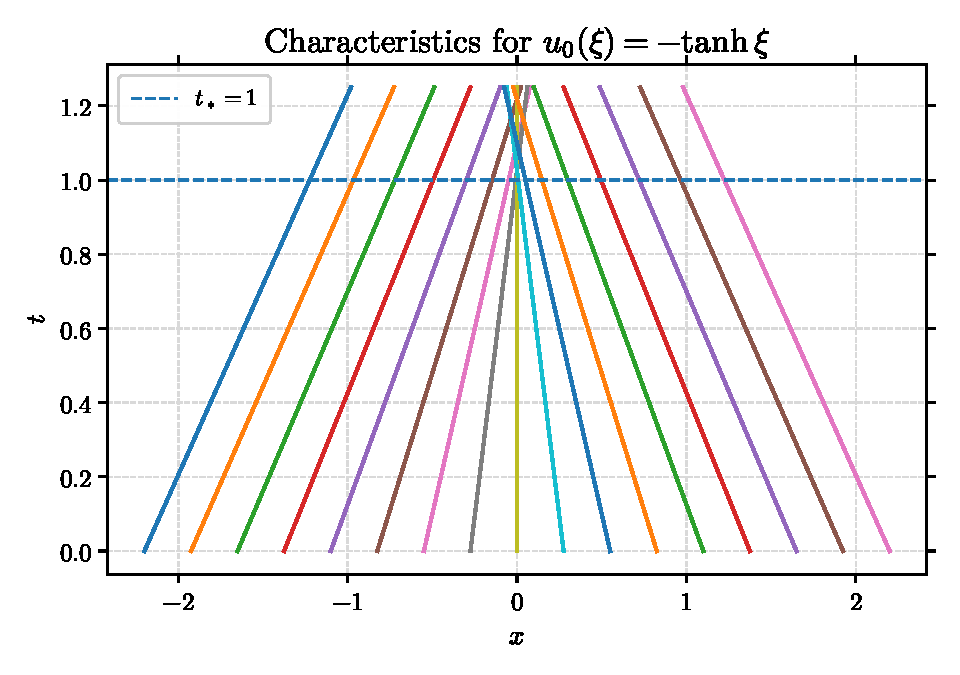
\includegraphics[width=0.78\textwidth]{content/MathSkills/figures/mathematical-physics/generated/burgers_characteristics.pdf}
\caption{无黏 Burgers 方程取 $u_0(\xi)=-\tanh\xi$ 时的特征线。由于 $\min u_0'=-1$，理论预言 $t_*=1$；图中正是在这条水平线附近首先出现特征线交叉。}
\label{fig:burgers-characteristic-crossing}
\end{figure}
经典解破裂后，Rankine--Hugoniot 条件和熵条件给出跳跃传播与唯一性选择。

无黏 Burgers 可以写成守恒律
\[
u_t+\left(\frac{u^2}{2}\right)_x=0.
\]
对一般守恒律
\[
u_t+f(u)_x=0,
\]
允许解在曲线 \(x=s(t)\) 上跳跃。设跳跃两侧极限为
\[
u_L=\lim_{x\uparrow s(t)}u(x,t),
\qquad
u_R=\lim_{x\downarrow s(t)}u(x,t).
\]
在跨越跳跃的小控制体上积分守恒律，并令控制体宽度趋于零，得到 Rankine--Hugoniot 条件
\begin{equation}
\boxed{
\dot s\,[u]=[f(u)]
},
\label{eq:rankine-hugoniot}
\end{equation}
其中
\[
[u]=u_L-u_R,
\qquad
[f]=f(u_L)-f(u_R).
\]
对 Burgers 的 \(f(u)=u^2/2\)，于是
\[
\boxed{
\dot s=\frac{u_L+u_R}{2}
}.
\]
这与前面黏性行波的速度
\[
c=\frac{v_1+v_2}{2}
\]
完全一致。也就是说，黏性冲击层在 \(\nu\downarrow0\) 时正好逼近守恒律弱解的激波速度。

但弱解并不唯一，还需熵条件选出物理解。对凸通量 Burgers 方程，压缩激波要求
\[
u_L>u_R.
\]
由于特征速度为 \(f'(u)=u\)，这等价于
\[
u_R<\dot s<u_L.
\]
两侧特征线都朝激波汇聚。若反过来 \(u_L<u_R\)，特征线从间断处向外发散，正确解不是反向激波，而是稀疏波扇形解。黏性极限 \(\nu\downarrow0^+\) 会自动选择满足熵条件的弱解，这就是“vanishing viscosity”方法的核心物理含义。

加入小黏性后，冲击被平滑成具有可估计厚度的内层。

Burgers 黏性行波
\[
u(\zeta)=\frac{u_L+u_R}{2}
-\frac{u_L-u_R}{2}
\tanh\!\left[
\frac{u_L-u_R}{4\nu}(\zeta-\zeta_0)
\right]
\]
显示冲击层的特征厚度为
\begin{equation}
\boxed{
\ell_{\mathrm shock}
\sim\frac{4\nu}{u_L-u_R}
}.
\label{eq:burgers-shock-width}
\end{equation}
这里近似号表示按 \(\tanh\) 自变量的倒数定义宽度尺度，而非某个唯一的几何宽度约定。它清楚给出两种趋势：黏性越强，过渡层越宽；跳跃幅度越大，非线性压缩越强，过渡层越窄。

与耗散正则化相对，KdV 保留一列守恒量并把能量重排到色散尺度。

KdV 孤子之所以能长期保持结构，不只因为行波方程恰好有 \(\operatorname{sech}^2\) 解。以标准形式
\[
u_t-6u u_x+u_{xxx}=0
\]
为例，它有无穷多守恒量。先直接推出最前面的三个。

把方程写成
\[
u_t+\partial_x(-3u^2+u_{xx})=0.
\]
若 \(u\) 及导数在无穷远充分衰减，则积分得到
\begin{equation}
\boxed{
I_1=\int_{-\infty}^{\infty}u\,\dd x,
\qquad
\frac{\dd I_1}{\dd t}=0
}.
\label{eq:kdv-conservation-1}
\end{equation}

再把方程乘 \(u\)：
\[
uu_t-6u^2u_x+u u_{xxx}=0.
\]
利用
\[
uu_t=\frac12(u^2)_t,
\]
\[
-6u^2u_x=-2(u^3)_x,
\]
以及
\[
uu_{xxx}
=\partial_x\left(u u_{xx}-\frac12u_x^2\right),
\]
得到局部守恒律
\[
\partial_t\frac{u^2}{2}
+\partial_x\left(
-2u^3+u u_{xx}-\frac12u_x^2
\right)=0.
\]
因此
\begin{equation}
\boxed{
I_2=\int u^2\,\dd x
}
\label{eq:kdv-conservation-2}
\end{equation}
守恒。

第三个守恒量可以取
\begin{equation}
\boxed{
I_3=\int\left(u^3+\frac12u_x^2\right)\dd x
}
\label{eq:kdv-conservation-3}
\end{equation}
对当前符号约定它也是时间不变量。验证时对 \(I_3\) 求导，代入 \(u_t=6uu_x-u_{xxx}\)，然后反复分部积分；所有边界项在衰减条件下消失，体积分项成对抵消。

这些守恒量限制了演化过程中质量、平方范数和更高阶“能量”在模态之间任意耗散。KdV 与 Burgers 的一个关键差别就在这里：Burgers 的黏性项会耗散平方范数，而 KdV 的色散项只重新分配波形，不直接耗散这些守恒量。


\section{耗散、色散与可控长波约化}
\label{sec:dissipative-dispersive-regularization}

接下来考察同一守恒律的两种正则化。

对标量守恒律可考虑
\begin{equation}
u_t+\partial_x f(u)
=\nu u_{xx}-\beta u_{xxx},
\qquad
\nu\ge0,
\label{eq:viscous-dispersive-conservation-law}
\end{equation}
其中 \(\nu\) 控制耗散，\(\beta\) 控制色散。假设解在无穷远充分衰减。将方程乘以 \(u\) 并积分。非线性项满足
\[
\int u\,\partial_xf(u)\,\dd x
=
\int\partial_xG(u)\,\dd x=0,
\qquad
G'(u)=u f'(u).
\]
黏性项给出
\[
\nu\int u u_{xx}\,\dd x
=-\nu\int u_x^2\,\dd x,
\]
而三阶色散项满足
\[
-\beta\int u u_{xxx}\,\dd x=0.
\]
因此
\begin{equation}
\frac{\dd}{\dd t}
\frac12\int u^2\,\dd x
=-\nu\int u_x^2\,\dd x\le0.
\label{eq:viscosity-dissipation-l2}
\end{equation}
这条式子精确地区分了两种正则化：黏性真正耗散 \(L^2\) 能量，色散则只把结构重新分配到不同尺度。Burgers 与 KdV 的不同长期行为首先来自这一算子级差异，而不是来自孤子公式的外形。

接下来考察Burgers 与 Hopf--Cole 精确线性化。

黏性 Burgers 方程
\begin{equation}
u_t+u u_x=\nu u_{xx},
\qquad \nu>0,
\label{eq:viscous-burgers}
\end{equation}
是耗散正则化的最简单非线性模型。令
\begin{equation}
u(x,t)=-2\nu\,\partial_x\ln Z(x,t),
\label{eq:hopf-cole-substitution}
\end{equation}
则原非线性方程精确化为热方程
\begin{equation}
Z_t=\nu Z_{xx}.
\label{eq:hopf-cole-heat}
\end{equation}
只要 \(Z>0\)，这个变换没有引入近似。若初值为 \(u_0(x)\)，则
\[
Z(x,0)
=Z_0(x)
=C\exp\left[
-\frac1{2\nu}
\int_{x_*}^xu_0(y)\,\dd y
\right].
\]
热核给出
\[
Z(x,t)=
\frac1{\sqrt{4\pi\nu t}}
\int_{\RR}
\exp\left[-\frac{(x-y)^2}{4\nu t}\right]
Z_0(y)\,\dd y,
\]
再由\eqnrefs{eq:hopf-cole-substitution} 恢复 \(u\)。因此 Burgers 的非线性初值问题被精确转化为线性热传播。

\begin{derivation}[Hopf--Cole 变换]
令
\[
q=\ln Z,
\qquad
u=-2\nu q_x.
\]
则
\[
u_t=-2\nu q_{xt},
\qquad
u_x=-2\nu q_{xx},
\qquad
u_{xx}=-2\nu q_{xxx}.
\]
代入\eqnrefs{eq:viscous-burgers}：
\[
-2\nu q_{xt}
+4\nu^2q_xq_{xx}
=-2\nu^2q_{xxx}.
\]
除以 \(-2\nu\) 后得到
\[
q_{xt}-2\nu q_xq_{xx}
=\nu q_{xxx}.
\]
注意
\[
2q_xq_{xx}=\partial_x(q_x^2),
\]
故
\[
\partial_x
\bigl(q_t-\nu q_{xx}-\nu q_x^2\bigr)=0.
\]
括号因此只依赖 \(t\)。把这一纯时间函数吸收到 \(Z\) 的时间依赖归一化中，可取
\[
q_t=\nu(q_{xx}+q_x^2).
\]
又因为
\[
q_t=\frac{Z_t}{Z},
\qquad
q_{xx}+q_x^2=\frac{Z_{xx}}{Z},
\]
所以
\[
Z_t=\nu Z_{xx}.
\]
反向代入同样成立，因此这是精确等价变换。
\end{derivation}

接下来考察弱非线性与弱色散必须同阶。

色散模型的关键不是先写下 KdV，而是从母系统识别两个彼此独立的小参数。对自由表面水波，振幅比
\[
\varepsilon=\frac{a}{h_0}
\]
控制非线性，而浅水参数
\[
\mu=\left(\frac{h_0}{L}\right)^2
\]
控制色散。只有在 distinguished limit
\[
\varepsilon=O(\mu)
\]
下，二次非线性与三阶色散才在同一个慢时间尺度上竞争；若两者阶数不同，最低阶模型会分别退化为无黏守恒律或近线性色散方程。

下面从精确自由边界 Euler 系统开始把这一约化链算清楚。

下面从精确自由表面方程出发，以无量纲控制参数依次推出 Boussinesq 系统与单向 KdV 近似。

前面用 $\varepsilon$ 与 $\mu$ 说明了 KdV 来自弱非线性与弱色散同阶竞争。若只从一个已经写好的 Boussinesq 方程开始，仍然看不出这两个小参数从哪里来。这里先把母问题写到精确层，再逐级进入近似。

考虑二维、无黏、不可压、无旋、忽略表面张力的自由表面水波。流体区域为
\[
-h_0<z<\eta(x,t),
\]
速度势记为 $\Phi(x,z,t)$。不可压与无旋给出区域内的 Laplace 方程
\[
\Phi_{xx}+\Phi_{zz}=0,
\qquad -h_0<z<\eta(x,t),
\]
平底边界条件为
\[
\Phi_z(x,-h_0,t)=0.
\]
自由表面上同时满足精确运动学条件与 Bernoulli 条件
\[
\eta_t+\Phi_x\eta_x-\Phi_z=0,
\]
\[
\Phi_t+\frac12(\Phi_x^2+\Phi_z^2)+g\eta=0,
\qquad z=\eta(x,t).
\]
此处仍是完整的自由表面 Euler--Dirichlet--Neumann 系统；浅水、小振幅与单向传播只在下述尺度展开中作为彼此独立的受控近似引入。

为了把“体内调和延拓”压缩到表面变量，定义表面势
\[
\psi(x,t)=\Phi(x,\eta(x,t),t)
\]
以及 Dirichlet--Neumann 算符
\[
G(\eta)\psi=(\Phi_z-\eta_x\Phi_x)_{z=\eta}.
\]
则自由边界 Euler 系统可等价写成 Zakharov 形式
\begin{equation}
\boxed{
\begin{aligned}
\eta_t&=G(\eta)\psi,\\
\psi_t+g\eta+\frac12\psi_x^2
&-\frac12\frac{\bigl(G(\eta)\psi+\eta_x\psi_x\bigr)^2}{1+\eta_x^2}=0.
\end{aligned}
}
\label{eq:zakharov-water-wave}
\end{equation}
这可以看成浅水 KdV 推导的精确理论起点：困难被集中到非线性、非局域算符 $G(\eta)$ 中。

现在才进入系统参数化。令典型波幅、静水深和水平尺度分别为 $a,h_0,L$，线性浅水波速为
\[
c_0=\sqrt{gh_0},
\]
并定义
\begin{equation}
\boxed{
\varepsilon=\frac{a}{h_0},
\qquad
\mu=\left(\frac{h_0}{L}\right)^2
}.
\label{eq:water-wave-small-parameters}
\end{equation}
$\varepsilon$ 控制自由表面非线性，$\mu$ 控制长波色散。具体无量纲化可取
\[
x=L\tilde x,
\qquad z=h_0\tilde z,
\qquad \eta=a\tilde\eta,
\qquad t=\frac{L}{c_0}\tilde t,
\]
并给速度势选择与 $aLc_0/h_0$ 同阶的尺度；随后把波浪号省略。此时 $\varepsilon,\mu$ 是方程中真正控制展开的两个无量纲参数，而不是事后从结果中辨认出来的系数。

对\cref{eq:zakharov-water-wave}中的 $G(\eta)$ 及非线性边界条件按 $(\varepsilon,\mu)$ 展开，会得到一族彼此经近恒等变量变换相关的 Boussinesq 系统。若取 distinguished limit
\[
\varepsilon=O(\mu)
\]
并只保留 $O(\varepsilon)$ 与 $O(\mu)$，则舍弃项为
\[
O(\varepsilon^2,\varepsilon\mu,\mu^2).
\]
选定一个标量变量并吸收 $\mu/\varepsilon=O(1)$ 到色散系数后，可把这一阶双向模型写成规范的 Boussinesq 型方程
\begin{equation}
\boxed{
u_{tt}-u_{xx}
-\varepsilon\Big[\alpha_{\mathrm B}(u^2)_{xx}+\beta_{\mathrm B}u_{xxxx}\Big]=0,
\qquad 0<\varepsilon\ll1
}.
\label{eq:boussinesq-canonical}
\end{equation}
其中 $\alpha_{\mathrm B}$ 是由变量选择和非线性展开确定的 $O(1)$ 系数，$\beta_{\mathrm B}$ 同时包含原问题中 $\mu/\varepsilon$ 的 $O(1)$ 比例因子。严格地说，左端等于一个 $O(\varepsilon^2)$ 的渐近残差；下面把这个残差统一记入被舍弃的高阶项，而不是把 Boussinesq 模型重新宣称成精确 Euler 方程。

当 $\varepsilon=0$ 时，\cref{eq:boussinesq-canonical}退化为一维波动方程
\[
u_{tt}-u_{xx}=0,
\]
其一般解由右行波 $F(x-t)$ 和左行波 $G(x+t)$ 叠加而成。若只研究一束主要向右传播、同时在长时间尺度上缓慢变形的波，就引入
\[
\xi=x-t,
\qquad
\tau=\varepsilon t.
\]
这里 $\xi$ 跟随线性右行波移动，而 $\tau$ 描述非线性和色散累积到 $O(1)$ 所需要的慢时间 $t=O(\varepsilon^{-1})$。

微分算符变为
\[
\partial_t=-\partial_\xi+\varepsilon\partial_\tau,
\qquad
\partial_x=\partial_\xi,
\]
从而
\[
\partial_t^2
=\partial_\xi^2-2\varepsilon\partial_\xi\partial_\tau
+\varepsilon^2\partial_\tau^2.
\]
设
\[
u(x,t;\varepsilon)=u_0(\xi,\tau)+\varepsilon u_1(\xi,\tau)+O(\varepsilon^2).
\]
于是
\[
u_{tt}-u_{xx}=-2\varepsilon u_{0,\xi\tau}+O(\varepsilon^2),
\]
而因为非线性和色散项本身已经带有 $\varepsilon$，在 $O(\varepsilon)$ 只需代入 $u_0$：
\[
(u^2)_{xx}=(u_0^2)_{\xi\xi}+O(\varepsilon),
\qquad
u_{xxxx}=u_{0,\xi\xi\xi\xi}+O(\varepsilon).
\]
代回\cref{eq:boussinesq-canonical}并除去共同因子 $\varepsilon$，得到
\[
-2u_{0,\xi\tau}-\alpha_{\mathrm B}(u_0^2)_{\xi\xi}
-\beta_{\mathrm B}u_{0,\xi\xi\xi\xi}=0.
\]
若波在 $|\xi|\to\infty$ 时趋于同一常值背景，为简便取该背景为零，对 $\xi$ 积分一次：
\[
-2u_{0,\tau}-\alpha_{\mathrm B}(u_0^2)_\xi
-\beta_{\mathrm B}u_{0,\xi\xi\xi}=0.
\]
利用 $(u_0^2)_\xi=2u_0u_{0,\xi}$，得到
\begin{equation}
\boxed{
u_{0,\tau}+\alpha_{\mathrm B}u_0u_{0,\xi}
+\frac{\beta_{\mathrm B}}{2}u_{0,\xi\xi\xi}=0
}.
\label{eq:boussinesq-to-kdv}
\end{equation}
这就是 KdV 型方程。

这个推导同时说明了每一项的渐近阶数：慢时间演化、二次非线性与三阶色散全部来自原方程的 $O(\varepsilon)$ 修正，因此必须同时保留。若把色散再假设小一个阶，最低阶将退化为无黏 Burgers 型方程并在有限时间产生梯度灾变；若把非线性小一个阶，则只剩线性色散方程。KdV 描述的正是两种效应在同一渐近阶上平衡的 distinguished limit。

还要注意近似的时间尺度。由于 $\tau=\varepsilon t$，\cref{eq:boussinesq-to-kdv}控制的是 $t=O(\varepsilon^{-1})$ 的慢演化。在这个时间尺度上，被舍去的 $O(\varepsilon^2)$ 项仍比保留项小一阶；若继续推到更长尺度，或者波幅增长到使 $\varepsilon u$ 不再小，就需要重新引入更高阶非线性、五阶色散或左右行波耦合。

若 $\alpha_{\mathrm B}\ne0$、$\beta_{\mathrm B}\ne0$，作尺度变换
\[
\xi=L_0X,
\qquad \tau=T_0T,
\qquad u_0=AU,
\]
则
\[
\frac{A}{T_0}U_T+\frac{\alpha_{\mathrm B}A^2}{L_0}UU_X
+\frac{\beta_{\mathrm B}A}{2L_0^3}U_{XXX}=0.
\]
选取 $A,L_0,T_0$ 使
\[
\frac{\alpha_{\mathrm B}AT_0}{L_0}=6,
\qquad
\frac{\beta_{\mathrm B}T_0}{2L_0^3}=1,
\]
便得到标准式
\[
U_T+6UU_X+U_{XXX}=0.
\]
选择另一振幅尺度也可把非线性系数归一化为 $1$，得到正文使用的
\[
u_t+uu_x+\beta_{\mathrm K}u_{xxx}=0.
\]
这些标准式之间只是尺度约定不同；真正具有物理内容的是非线性项与三阶色散项处于同一渐近阶。

最后把抽象系数代回最常见的无表面张力浅水高程方程。对自由表面位移 $\eta(x,t)$，一阶 KdV 近似在实验坐标中可写成
\begin{equation}
\boxed{
\eta_t+c_0\eta_x+\frac{3c_0}{2h_0}\eta\eta_x
+\frac{c_0h_0^2}{6}\eta_{xxx}=0,
\qquad c_0=\sqrt{gh_0}
}.
\label{eq:physical-shallow-water-kdv}
\end{equation}
进入随线性波移动的坐标 $X=x-c_0t$、$T=t$，再代入
\[
\eta=aU,
\qquad X=L\xi,
\qquad \tau=\frac{\varepsilon c_0}{L}T,
\qquad
\varepsilon=\frac{a}{h_0},
\qquad
\mu=\frac{h_0^2}{L^2},
\]
逐项得到
\[
U_\tau+\frac32UU_\xi+\frac{\mu}{6\varepsilon}U_{\xi\xi\xi}=0.
\]
现在可以直接看见 distinguished limit 的作用：只有在 $\mu/\varepsilon=O(1)$ 时，非线性与色散才在同一慢时间上同时保留。这个有量纲特例与前面的抽象 Boussinesq--KdV 约化是同一条逻辑链，只是最后把抽象系数具体化成了 $g,h_0,a,L$。


接下来考察近似的控制参数与失效边界。

Burgers、KdV 和 NLS 都不是“非线性 PDE 的代表公式表”，而是不同尺度平衡下的有效方程。以 KdV 为例，\(\varepsilon\sim\mu\ll1\) 保证弱非线性、弱色散同阶，单向近似又要求反向传播分量在所考虑时间尺度内不积累到主阶。若演化推进到更长的 \(O(\varepsilon^{-2})\) 时间，或谱宽变大使更高阶色散不可忽略，就必须加入更高阶项或回到双向模型。

同样，Burgers 的 vanishing-viscosity 极限要求 \(\nu\to0^+\) 与空间分辨尺度协调；在固定数值网格上直接令 \(\nu=0\) 并不能自动得到 entropy solution。有效模型的可靠性来自控制参数和误差阶，而不是来自某个特解与实验曲线“看起来相似”。

\section{守恒律、Hamilton 结构与反散射的统一视角}

前两节已经建立一般演化、守恒律以及 KdV 的受控长波来源。可积情形还具有更强的 Hamilton、Lax 与散射数据结构；这些结构不是从某个孤子外形反推出来的技巧，而是非线性演化本身的额外代数约束。

接下来考察Hamiltonian PDE 与 KdV 的第一 Poisson 结构。

有限维 Hamilton 系统的核心不是某组特殊正则坐标，而是“状态空间上的反对称 Poisson 算子把能量梯度变成动力学”。这一结构在无穷维中仍可保留。设状态 $u$ 属于函数空间 $X$，泛函 $H[u]$ 的一阶变分写成
\[
\delta H[u;\eta]
=\left\langle \frac{\delta H}{\delta u},\eta\right\rangle.
\]
若存在反对称算子 $J(u)$，满足适当定义域条件并使诱导括号满足 Jacobi 恒等式，则
\begin{equation}
 u_t=J(u)\frac{\delta H}{\delta u}
\label{eq:general-hamiltonian-pde}
\end{equation}
称为 Hamiltonian PDE。对两个泛函 $F,G$ 定义
\begin{equation}
\{F,G\}[u]
:=\left\langle
\frac{\delta F}{\delta u},
J(u)\frac{\delta G}{\delta u}
\right\rangle.
\label{eq:functional-poisson-bracket}
\end{equation}
则沿\eqnrefs{eq:general-hamiltonian-pde}
\[
\frac{\dd F}{\dd t}=\{F,H\}.
\]
特别地，由 $J^*=-J$，
\[
\frac{\dd H}{\dd t}
=\left\langle \frac{\delta H}{\delta u},
J\frac{\delta H}{\delta u}\right\rangle=0.
\]
反对称性只保证 $\{H,H\}=0$；要使\eqnrefs{eq:functional-poisson-bracket}真正成为 Poisson 括号，还必须满足 Jacobi 恒等式。常系数微分算子 $J=\partial_x$ 在周期或快速衰减边界条件下是最简单的例子。

现在把一般结构代入 KdV。仍采用
\[
u_t-6u u_x+u_{xxx}=0.
\]
定义泛函
\[
H[u]=\int_{-\infty}^{\infty}
\left(u^3+\frac12u_x^2\right)\dd x.
\]
对变分 \(u\mapsto u+\varepsilon\eta\)，有
\[
\begin{aligned}
\delta H
&=\left.\frac{\dd}{\dd\varepsilon}
H[u+\varepsilon\eta]\right|_{\varepsilon=0}\\
&=\int\left(3u^2\eta+u_x\eta_x\right)\dd x\\
&=\int\left(3u^2-u_{xx}\right)\eta\,\dd x,
\end{aligned}
\]
其中最后一步使用分部积分并假设边界项消失。因此泛函导数为
\[
\frac{\delta H}{\delta u}=3u^2-u_{xx}.
\]
KdV 可以写成
\begin{equation}
\boxed{
u_t=\partial_x\frac{\delta H}{\delta u}}
\label{eq:kdv-hamiltonian}
\end{equation}
即
\[
u_t=\partial_x(3u^2-u_{xx})=6u u_x-u_{xxx}.
\]

若定义 Poisson 括号
\[
\{F,G\}
=\int\frac{\delta F}{\delta u}
\partial_x\frac{\delta G}{\delta u}\,\dd x,
\]
则任意泛函沿 KdV 流的变化为
\[
\frac{\dd F}{\dd t}=\{F,H\}.
\]
特别地
\[
\frac{\dd H}{\dd t}=\{H,H\}=0,
\]
因为 \(\partial_x\) 在衰减边界条件下是反对称算符。于是前面第三个守恒量不仅“碰巧守恒”，而是 KdV Hamiltonian 本身。

接下来考察Lax 对为什么意味着等谱演化。

前面有
\[
L_t=[B,L].
\]
设
\[
L\psi=\lambda\psi,
\]
并令辅助函数随时间满足
\[
\psi_t=B\psi.
\]
对本征方程求时间导数：
\[
L_t\psi+L\psi_t
=\dot\lambda\psi+\lambda\psi_t.
\]
代入 \(L_t=[B,L]\) 与 \(\psi_t=B\psi\)：
\[
(BL-LB)\psi+LB\psi
=\dot\lambda\psi+\lambda B\psi.
\]
左边化为
\[
BL\psi=\lambda B\psi.
\]
因此
\[
\dot\lambda\psi=0.
\]
对非零本征函数得到
\begin{equation}
\boxed{\dot\lambda=0}.
\label{eq:lax-isospectral}
\end{equation}
这就是“等谱变形”的直接推导。KdV 的非线性时间演化改变势函数 \(u(x,t)\)，却保持一维 Schrodinger 算符
\[
L(t)=-\partial_x^2+u(x,t)
\]
的谱数据不变。

更抽象地，如果存在可逆算符 \(U(t)\) 使
\[
L(t)=U(t)L(0)U(t)^{-1},
\]
那么相似变换当然保持谱。Lax 方程正是这种等谱流的微分形式：若 \(U_t=BU\)，就有
\[
\frac{\dd}{\dd t}
\bigl(UL(0)U^{-1}\bigr)
=[B,L].
\]

接下来考察从散射数据到一孤子。

对快速衰减势 \(u(x,t)\)，考虑谱问题
\[
-\psi_{xx}+u(x,t)\psi=k^2\psi.
\]
连续谱位于 \(k^2\ge0\)，而负本征值写成
\[
\lambda_n=-\kappa_n^2,
\qquad \kappa_n>0.
\]
散射数据包含反射系数、离散本征值 \(-\kappa_n^2\) 以及相应归一化常数。Lax 等谱性说明 \(\kappa_n\) 不随时间改变，而辅助方程决定其余散射数据只获得简单指数时间因子。于是原来复杂的非线性 PDE 演化被搬到了``散射数据空间''中，那里时间演化变成简单的指数或相位因子。

最简单的 reflectionless 情形只有一个离散本征值 \(-\kappa^2\) 且反射系数为零。与其只写“逆散射重构得到孤子”，不如把最短的 Marchenko 重构真正做完。

对快速衰减势，逆散射的一种形式是 Gel'fand--Levitan--Marchenko 方程
\begin{equation}
K(x,y,t)+F(x+y,t)
+\int_x^\infty K(x,s,t)F(s+y,t)\,\dd s=0,
\qquad y\ge x,
\label{eq:glm-marchenko}
\end{equation}
重构势由
\begin{equation}
\boxed{
 u(x,t)=-2\frac{\partial}{\partial x}K(x,x,t)
}
\label{eq:marchenko-potential-reconstruction}
\end{equation}
给出。一般的 \(F\) 同时包含连续谱反射数据与离散谱数据；这就是逆散射阶段的形式精确表达。

只有一个束缚态且反射系数为零时，\(F\) 简化为
\[
F(z,t)=c(t)\ee^{-\kappa z},
\qquad \kappa>0.
\]
由于右端只有一个指数模式，可以尝试
\[
K(x,y,t)=-A(x,t)\ee^{-\kappa y}.
\]
代入 \cref{eq:glm-marchenko}，并提取公共因子 \(\ee^{-\kappa y}\)，得到
\[
-A+c\ee^{-\kappa x}
-Ac\int_x^\infty\ee^{-2\kappa s}\,\dd s=0.
\]
积分为
\[
\int_x^\infty\ee^{-2\kappa s}\,\dd s
=\frac{\ee^{-2\kappa x}}{2\kappa},
\]
因此
\[
A(x,t)
=\frac{c(t)\ee^{-\kappa x}}
{1+\dfrac{c(t)}{2\kappa}\ee^{-2\kappa x}}.
\]
于是
\begin{equation}
K(x,x,t)
=-\frac{c(t)\ee^{-2\kappa x}}
{1+\dfrac{c(t)}{2\kappa}\ee^{-2\kappa x}}.
\label{eq:marchenko-one-bound-kernel}
\end{equation}

令
\[
z(x,t)=\frac{c(t)}{2\kappa}\ee^{-2\kappa x},
\]
则
\[
K(x,x,t)=-2\kappa\frac{z}{1+z},
\qquad
z_x=-2\kappa z.
\]
因此
\[
\frac{\partial K(x,x,t)}{\partial x}
=4\kappa^2\frac{z}{(1+z)^2},
\]
由 \cref{eq:marchenko-potential-reconstruction} 得
\begin{equation}
 u(x,t)
=-8\kappa^2\frac{z}{(1+z)^2}.
\label{eq:ist-z-form}
\end{equation}
若把归一化常数参数化为
\[
\frac{c(t)}{2\kappa}
=\exp\bigl(2\kappa x_0(t)\bigr),
\]
则
\[
z=\exp[-2\kappa(x-x_0(t))].
\]
利用恒等式
\[
\operatorname{sech}^2\eta
=\frac{4\ee^{-2\eta}}{(1+\ee^{-2\eta})^2},
\]
\cref{eq:ist-z-form} 化为
\[
 u(x,t)
=-2\kappa^2
\operatorname{sech}^2\!\bigl[\kappa(x-x_0(t))\bigr].
\]

还需确定 \(x_0(t)\)。对当前符号的 KdV Lax 对，无穷远处辅助算符退化为 \(-4\partial_x^3\)，离散谱归一化常数按
\[
c(t)=c(0)\ee^{8\kappa^3t}
\]
演化。因此
\[
 x_0(t)=4\kappa^2t+x_0(0),
\]
最终得到
\begin{equation}
\boxed{
 u(x,t)
=-2\kappa^2
\operatorname{sech}^2
\bigl[\kappa(x-4\kappa^2t-x_0)\bigr]
}.
\label{eq:kdv-ist-one-soliton}
\end{equation}
这与前面 Hirota 变换对
\[
 u_t-6u u_x+u_{xxx}=0
\]
得到的一孤子完全一致。这里现在可以看见“reflectionless 势为什么是 \(\operatorname{sech}^2\)”：它来自只有一个指数离散谱项时 Marchenko 积分方程的秩一精确解，而不是从孤子外形反推出来的猜测。

因此一孤子可以从三个角度得到：
\[
\text{行波 ODE}
\longleftrightarrow
\text{Hirota tau 函数}
\longleftrightarrow
\text{reflectionless Schrodinger 势}.
\]
三种方法给出同一个解，但揭示的信息不同。行波法给出速度--振幅关系；Hirota 法最适合多孤子代数；逆散射揭示为什么碰撞前后谱参数 \(\kappa_n\) 不变。

在一孤子的谱重构之后，多孤子解还能显示散射前后位置参数的有限相移。以二孤子 tau 函数为例，

取
\[
\tau=1+\ee^{\eta_1}+\ee^{\eta_2}
+A_{12}\ee^{\eta_1+\eta_2},
\]
\[
A_{12}=
\left(\frac{k_1-k_2}{k_1+k_2}\right)^2,
\qquad k_1>k_2>0,
\]
并取
\[
\eta_i=2k_i(x-4k_i^2t-x_{i0}).
\]
对快速孤子 \(k_1\)，沿其轨道 \(x\sim4k_1^2t\)。当 \(t\to-\infty\) 时，\(\eta_2\to-\infty\)，所以
\[
\tau\sim1+\ee^{\eta_1}.
\]
孤子中心由 \(\eta_1=0\) 给出。碰撞后 \(t\to+\infty\) 时，\(\eta_2\to+\infty\)，提取无关的线性指数因子：
\[
\tau\sim \ee^{\eta_2}
\left(1+A_{12}\ee^{\eta_1}\right).
\]
由于 \((\ln \ee^{\eta_2})_{xx}=0\)，它不改变 \(u=-2(\ln\tau)_{xx}\)。新的中心条件是
\[
A_{12}\ee^{\eta_1}=1,
\qquad
\eta_1=-\ln A_{12}.
\]
因此快速孤子的前向相移为
\begin{equation}
\boxed{
\Delta x_1
=-\frac{\ln A_{12}}{2k_1}>0
}.
\label{eq:kdv-fast-phase-shift}
\end{equation}

同理，沿慢孤子轨道 \(x\sim4k_2^2t\)，碰撞前 \(\eta_1\to+\infty\)，碰撞后 \(\eta_1\to-\infty\)。得到
\begin{equation}
\boxed{
\Delta x_2
=\frac{\ln A_{12}}{2k_2}<0
}.
\label{eq:kdv-slow-phase-shift}
\end{equation}
所以快孤子被向前推进，慢孤子被向后延迟；碰撞改变位置参数，却不改变各自 \(k_i\)、速度 \(4k_i^2\) 与振幅 \(2k_i^2\) 的绝对值。这就是弹性孤子散射的定量内容。\\figref{fig:kdv-two-soliton-scattering} 给出了碰撞前、碰撞中与碰撞后的三个定量截面。


\begin{figure}[htbp]
\centering
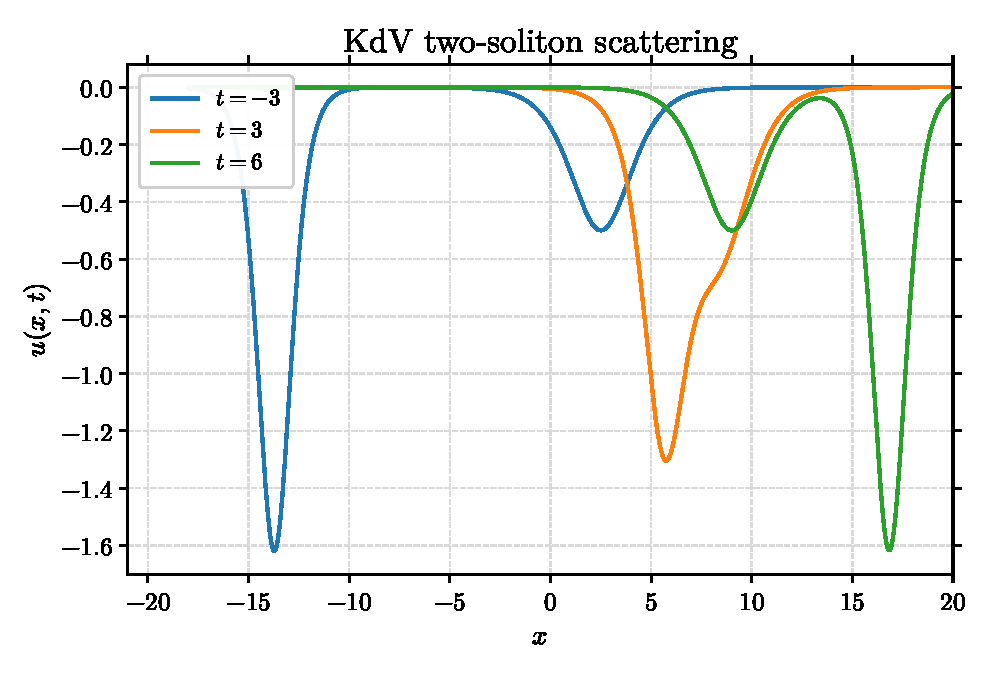
\includegraphics[width=0.79\textwidth]{content/MathSkills/figures/mathematical-physics/generated/kdv_two_soliton.pdf}
\caption{标准符号 $u_t-6uu_x+u_{xxx}=0$ 下二孤子 tau 函数给出的三个时刻截面。碰撞区域中波形强烈叠加，但远离碰撞后又恢复为由 $k_1,k_2$ 决定的两条孤子，只留下中心位置的相移。}
\label{fig:kdv-two-soliton-scattering}
\end{figure}

接下来考察Sine--Gordon kink 的拓扑荷与能量。

将 Sine--Gordon 归一化为
\[
\phi_{tt}-\phi_{xx}+\sin\phi=0.
\]
其势能密度
\[
V(\phi)=1-\cos\phi
\]
在
\[
\phi=2\pi n,
\qquad n\in\mathbb Z
\]
有无限多个等价真空。对有限能量构型，\(x\to\pm\infty\) 时场必须趋于某个真空，因此可以定义拓扑荷
\begin{equation}
\boxed{
Q=\frac{\phi(+\infty)-\phi(-\infty)}{2\pi}
}.
\label{eq:sine-gordon-topological-charge}
\end{equation}
对 kink 有 \(Q=1\)，antikink 有 \(Q=-1\)。连续、有限能量的局部变形不能改变无穷远真空编号，所以 \(Q\) 是拓扑不变量。

静态 kink
\[
\phi_K(x)=4\arctan \ee^{x-x_0}
\]
满足
\[
\phi_K'(x)=2\operatorname{sech}(x-x_0).
\]
还可直接验证
\[
1-\cos\phi_K
=2\operatorname{sech}^2(x-x_0).
\]
静态能量为
\[
E=\int_{-\infty}^{\infty}
\left[
\frac12\phi_x^2+1-\cos\phi
\right]\dd x.
\]
代入 kink：
\[
E_K
=\int 4\operatorname{sech}^2(x-x_0)\,\dd x
=8.
\]
因此
\begin{equation}
\boxed{E_{\mathrm{kink}}=8}
\label{eq:sine-gordon-kink-energy}
\end{equation}
在当前无量纲归一化下成立。

Lorentz 不变性又允许把静态 kink boost 成速度 \(|v|<1\) 的移动 kink：
\[
\phi(x,t)
=4\arctan\exp\!\left[
\gamma(x-vt-x_0)
\right],
\qquad
\gamma=\frac1{\sqrt{1-v^2}}.
\]
它的总能量变为
\[
E=8\gamma.
\]
因此 kink 的静能量像一个有效静质量；这也是拓扑孤子呈现粒子性质的一个直接表现。

\section{非线性 Schrodinger 方程：从一般窄带波包到包络孤子}

NLS 在这里不作为凭经验写下的另一个非线性方程，而是作为一般弱非线性色散波包的首阶慢包络方程出现。先设某个平移不变系统在线性化后有一条色散支
\[
\omega=\omega(k),
\]
并选定载波 $(k_0,\omega_0)$，其中 $\omega_0=\omega(k_0)$。进一步假设该载波模是简单本征模，二次谐波与零频模不存在共振，而且色散关系在 $k_0$ 附近足够光滑。若这些条件失效，首个闭合包络系统可能是耦合模方程、二次非线性包络方程或更高阶 NLS，而不能继续使用单标量三次 NLS。

若载波振幅为 $O(\varepsilon)$、频谱集中在 $k_0$ 附近，就引入快相位与慢变量
\[
\theta=k_0x-\omega_0t,
\qquad
X=\varepsilon(x-v_gt),
\qquad
T=\varepsilon^2t,
\]
以及多尺度展开
\[
q(x,t)=\varepsilon\bigl[A(X,T)r\ee^{\ii\theta}+\text{c.c.}\bigr]
+\varepsilon^2q_2+\varepsilon^3q_3+\cdots.
\]
这里 $r$ 是线性本征模；若原系统只有一个标量场，可取 $r=1$。

把展开代回母系统后，$O(\varepsilon)$ 只重复线性色散关系 $\omega_0=\omega(k_0)$。在 $O(\varepsilon^2)$，一阶谐波若不消失会产生与载波同频的 secular forcing；可解条件固定群速度
\[
\boxed{v_g=\omega'(k_0)}.
\]
到了 $O(\varepsilon^3)$，线性色散曲率产生 $A_{XX}$，三阶共振非线性产生 $|A|^2A$。把这一阶的一阶谐波投影到伴随线性本征模上，得到一般包络方程
\begin{equation}
\boxed{
\ii A_T+\frac12\omega''(k_0)A_{XX}+\Gamma|A|^2A=0
}.
\label{eq:nls-envelope-general}
\end{equation}
其中 $\Gamma$ 不是由色散关系单独决定的常数；它必须从原系统的二次/三次非线性、二次谐波修正以及本征模归一化中计算。换言之，$\omega''(k_0)$ 是线性理论的参数代入，而 $\Gamma$ 是非线性共振投影的结果，两者来源不同。

定义
\begin{equation}
D=\frac12\omega''(k_0),
\qquad
\chi=\Gamma,
\label{eq:nls-coefficient-identification}
\end{equation}
并把慢包络 $A$ 重命名为 $\psi$。从这里开始再把慢变量 $(X,T)$ 简记为 $(x,t)$，得到后文使用的标准 NLS
\begin{equation}
\boxed{
\ii\psi_t+D\psi_{xx}+\chi|\psi|^2\psi=0
}.
\label{eq:nls-general}
\end{equation}
这个重命名只是排版简化；本节余下的 $x,t$ 都表示包络慢变量，而不是母方程的快坐标。NLS 控制 $X=O(1),T=O(1)$，即原变量中 $O(\varepsilon^{-1})$ 的空间调制尺度和 $O(\varepsilon^{-2})$ 的演化时间。若频谱不再窄带、$\omega''(k_0)$ 接近零而需要更高阶色散，或非线性使 $\varepsilon|A|$ 不再小，这个三次 NLS 截断会失效。

为了看清一般系数怎样代入具体母方程，考虑非线性 Klein--Gordon 模型
\begin{equation}
q_{tt}-c^2q_{xx}+\omega_*^2q+\lambda q^3=0.
\label{eq:nlkg-parent-nls}
\end{equation}
其精确线性色散关系是
\[
\omega(k)=\sqrt{\omega_*^2+c^2k^2}.
\]
取
\[
q=\varepsilon\left[A(X,T)\ee^{\ii\theta}+A^*(X,T)\ee^{-\ii\theta}\right]+O(\varepsilon^3),
\]
\[
\theta=k_0x-\omega_0t,
\qquad
X=\varepsilon(x-v_gt),
\qquad
T=\varepsilon^2t.
\]
在 $O(\varepsilon^2)$，$\ee^{\ii\theta}$ 的系数为
\[
2\ii(\omega_0v_g-c^2k_0)A_X,
\]
所以
\[
v_g=\frac{c^2k_0}{\omega_0}=\omega'(k_0).
\]
在 $O(\varepsilon^3)$，$\ee^{\ii\theta}$ 的共振系数为
\[
-2\ii\omega_0A_T+(v_g^2-c^2)A_{XX}+3\lambda|A|^2A.
\]
令其为零并除以 $-2\omega_0$，得到
\[
\ii A_T+\frac{c^2-v_g^2}{2\omega_0}A_{XX}
-\frac{3\lambda}{2\omega_0}|A|^2A=0.
\]
而
\[
\frac{c^2-v_g^2}{2\omega_0}
=\frac12\omega''(k_0)
=\frac{c^2\omega_*^2}{2\omega_0^3}.
\]
因此这个具体系统给出
\begin{equation}
\boxed{
D=\frac{c^2\omega_*^2}{2\omega_0^3},
\qquad
\chi=-\frac{3\lambda}{2\omega_0}
}.
\label{eq:nlkg-to-nls-coefficients}
\end{equation}
这就是从一般包络系数到具体系统参数的一次完整代入；后面的调制不稳定和明孤子条件 $D\chi>0$，在这个母模型中进一步等价于 $\lambda<0$。

接下来考察平面波与非线性频移。

取空间均匀解
\[
\psi(x,t)=A \ee^{\ii \Omega t},
\qquad A>0.
\]
代入 \cref{eq:nls-general} 得
\[
-\Omega A+\chi A^3=0,
\]
所以
\[
\boxed{\Omega=\chi A^2}.
\]
非线性把相位旋转频率改成振幅相关量。这是后面调制不稳定和包络孤子形成的最简单来源。

接下来考察调制不稳定的线性分析。

令
\[
\psi=(A+\rho)\ee^{\ii \chi A^2t},
\qquad |\rho|\ll A.
\]
保留 \(\rho\) 的一阶项。利用
\[
|A+\rho|^2(A+\rho)
=A^3+A^2(2\rho+\rho^*)+O(|\rho|^2),
\]
消去背景方程后得到
\[
i\rho_t+D\rho_{xx}
+\chi A^2(\rho+\rho^*)=0.
\]
写
\[
\rho=a+ib,
\]
其中 \(a,b\) 为实函数，则
\[
-b_t+D a_{xx}+2\chi A^2a=0,
\]
\[
a_t+D b_{xx}=0.
\]
取 Fourier 模式
\[
a,b\propto \ee^{\ii (Kx-\Omega t)},
\]
线性方程组存在非零解要求行列式为零，得到
\begin{equation}
\boxed{
\Omega^2
=D^2K^4-2D\chi A^2K^2
}.
\label{eq:nls-modulational-dispersion}
\end{equation}

若 \(D\chi>0\)，则当
\[
0<K^2<\frac{2\chi A^2}{D}
\]
（按 \(D,\chi\) 同号理解）时右端为负，\(\Omega\) 变成纯虚数，扰动指数增长。这就是聚焦 NLS 的调制不稳定。若 \(D\chi<0\)，右端对所有实 \(K\) 都非负，均匀平面波在线性层面没有这种长波调制不稳定。

接下来考察聚焦 NLS 的明孤子。

在 \(D\chi>0\) 时寻找局域包络。取
\[
\psi(x,t)=F(\xi)\ee^{\ii (kx-\omega t)},
\qquad
\xi=x-vt,
\]
并要求 \(F\) 为实函数。代入方程，分别收集虚部和实部。虚部为
\[
(-v+2Dk)F'=0.
\]
非平凡局域解因此要求
\begin{equation}
\boxed{v=2Dk}.
\label{eq:nls-galilean-velocity}
\end{equation}
实部为
\[
D F''+(\omega-Dk^2)F+\chi F^3=0.
\]
取
\[
F(\xi)=A\operatorname{sech}(\kappa\xi).
\]
由恒等式
\[
\frac{\dd^2}{\dd\xi^2}\operatorname{sech}(\kappa\xi)
=\kappa^2\operatorname{sech}(\kappa\xi)
-2\kappa^2\operatorname{sech}^3(\kappa\xi)
\]
得到
\[
F''=\kappa^2F-\frac{2\kappa^2}{A^2}F^3.
\]
逐项比较 \(F\) 与 \(F^3\) 的系数：
\[
D\kappa^2+\omega-Dk^2=0,
\]
\[
\chi-\frac{2D\kappa^2}{A^2}=0.
\]
所以
\[
A^2=\frac{2D\kappa^2}{\chi},
\qquad
\omega=Dk^2-D\kappa^2.
\]
于是明孤子为
\begin{equation}
\boxed{
\psi(x,t)
=\sqrt{\frac{2D}{\chi}}\,\kappa
\operatorname{sech}[\kappa(x-2Dkt-x_0)]
\exp\!\left\{
i\bigl[kx-(Dk^2-D\kappa^2)t+\phi_0\bigr]
\right\}
}.
\label{eq:nls-bright-soliton}
\end{equation}
其中要求 \(D/\chi>0\)，正是聚焦条件。

振幅与宽度不是独立参数：
\[
A=\sqrt{\frac{2D}{\chi}}\,\kappa,
\qquad
L\sim\kappa^{-1}.
\]
包络越高，越窄。这是色散与自聚焦非线性平衡的直接结果。

接下来考察NLS 的三个基本守恒量。

在足够快衰减的边界条件下，NLS 守恒
\[
N=\int_{-\infty}^{\infty}|\psi|^2\,\dd x,
\]
\[
P=\operatorname{Im}
\int_{-\infty}^{\infty}\psi^*\psi_x\,\dd x,
\]
以及 Hamiltonian
\begin{equation}
\boxed{
H=\int_{-\infty}^{\infty}
\left(
D|\psi_x|^2-\frac{\chi}{2}|\psi|^4
\right)\dd x
}.
\label{eq:nls-hamiltonian}
\end{equation}

以 \(N\) 为例，
\[
\frac{\dd N}{\dd t}
=\int(\psi_t\psi^*+\psi\psi_t^*)\,\dd x.
\]
由 NLS 与其共轭式
\[
\psi_t=\ii D\psi_{xx}+\ii\chi|\psi|^2\psi,
\]
\[
\psi_t^*=-\ii D\psi_{xx}^*-\ii\chi|\psi|^2\psi^*,
\]
非线性项直接相消，剩下
\[
\frac{\dd N}{\dd t}
=iD\int(\psi_{xx}\psi^*-\psi\psi_{xx}^*)\,\dd x.
\]
而
\[
\psi_{xx}\psi^*-\psi\psi_{xx}^*
=\partial_x(\psi_x\psi^*-\psi\psi_x^*),
\]
所以边界项消失后
\[
\boxed{\frac{\dd N}{\dd t}=0}.
\]

同样的方法可验证 \(P\) 与 \(H\) 守恒。于是 NLS 与 KdV 再次形成平行结构：可积方程的特殊性不只是存在某个漂亮特解，而是存在一整套相容的守恒律、谱结构与多孤子散射机制。

